\documentclass[10pt]{article}
%\usepackage{wallpaper}
\usepackage[spanish]{babel}
\usepackage[utf8]{inputenc}
\usepackage[top=1in, bottom=1.0in, left=1.in, right=1.in]{geometry}

\usepackage{amsmath}
\usepackage{graphicx}
\usepackage{animate}
\usepackage{amssymb}
\usepackage{gensymb}
\usepackage[makeroom]{cancel}
\usepackage{mathtools}% Loads amsmath
\usepackage{tikz}

\newcommand{\angstrom}{\text{\normalfont\AA}}
\newlength\myheight
\newcommand*\ccircled[1]{\settowidth{\myheight}{#1}%
    \raisebox{-.1\myheight}{\tikz[baseline=(char.base)]{%
        \node[shape=circle,draw,minimum size=1.5em,inner sep=1pt](char){#1};}}}
        
\pagestyle{empty}
\setlength\parindent{0pt}

\begin{document}

%\vspace{1.5cm}
%\hfill{Buenos Aires, \today} \\

\begin{center}
 {\large \bf Estructura Electrónica de Materias: \\
 Cálculo desde primeros principios} \\
 
 \vspace{0.25cm}
 Guía Práctica N\degree 3
\end{center}

\vspace{0.5cm}
1. Para el valor experimental del parámetro de red, el estudio 
de convergencia de la energía total en {\verb k } resulta 
\begin{verbatim}
k  Energía total (eV)
2  -5.332352
4  -5.410362
6  -5.411693
8  -5.411816
\end{verbatim}
Así, la convergencia de la energía total en el rango de 0.001 eV se 
da para {\verb k=6 }.

\vspace{0.5cm}
2. Para 6 puntos en la zona de Brillouin, el estudio de convergencia 
de la energía total variando el valor de energías de ondas planas 
dado por {\verb ENCUT }
resulta 
\begin{verbatim}
ENCUT  Energía total (eV)
240 -5.411693
270 -5.417335
300 -5.420325
330 -5.421652
360 -5.422537
380 -5.422960
400 -5.423190
\end{verbatim}
La convergencia de la energía total en el rango de 0.001 eV se 
da para {\verb ENCUT=360 }.

\vspace{0.5cm}
3. Variando el parámetro de red {\verb ALAT } con {\verb k=6 } y 
{\verb ENCUT=460 }, desde {\verb ini= } $0.8\,a_{\mathrm{exp}}$ 
hasta {\verb fin= } $1.2\,a_{\mathrm{exp}}$.
\begin{verbatim}
4.4 10.650 -1.682994
4.6 12.165 -3.236655
4.8 13.825 -4.275415
5.0 15.625 -4.925580
5.2 17.575 -5.279724
5.3 18.610 -5.371074
5.4 19.685 -5.416526
5.45 20.235 -5.424330
5.5 20.795 -5.423298
5.6 21.950 -5.397779
5.7 23.150 -5.345616
5.9 25.670 -5.180627
6.1 28.375 -4.961070
6.3 31.255 -4.711050
6.5 34.330 -4.447268
\end{verbatim}

% \vspace{0.5cm}
\newpage
5. 
\begin{figure}[h]
 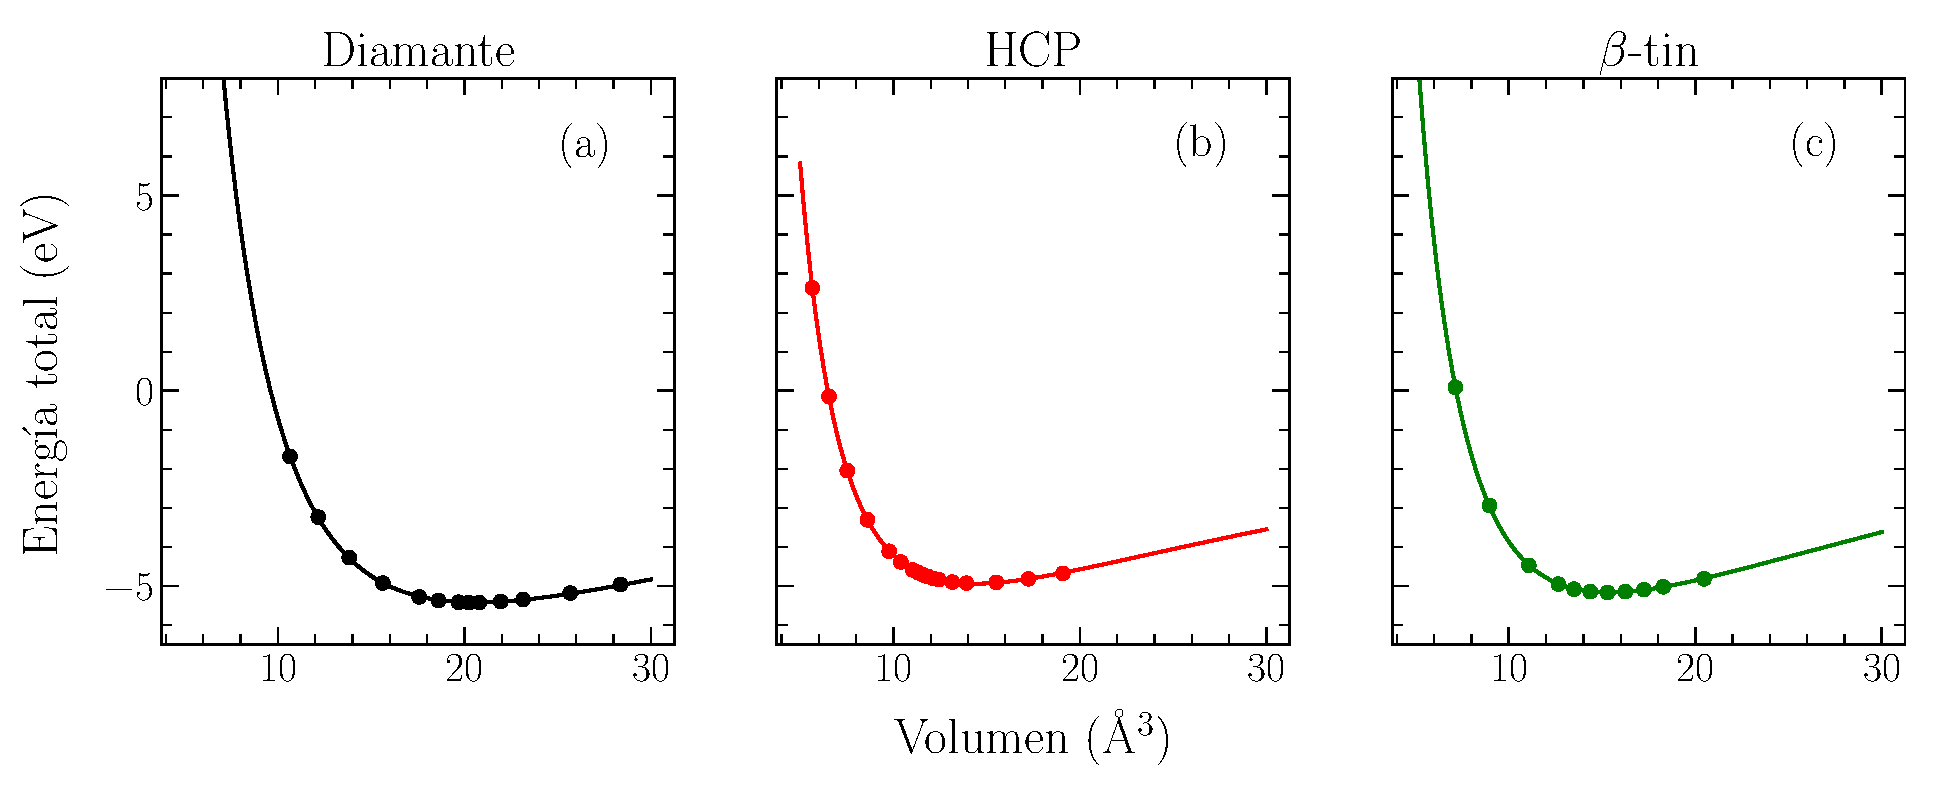
\includegraphics[width=\textwidth]{Si/punto5.eps}
\end{figure}
Las puntos en las figuras (a), (b) y (c) corresponden a los valores
de energía total en función del volumen de la celda para el silicio 
en sus estructuras diamante, hcp y $\beta$--tin, respectivamente.
Ajustando los puntos obtenidos con la función de estado de 
Birch--Murnaghan, los valores de energía mínima, módulo de volumen, 
volumen de equilibrio y derivada de $B0$ en función de V resultaron:
\begin{verbatim}
Parámetros de diamante:
E0 = -5.4199
B0 = 0.5201
V0 = 20.6127
B0' = 4.0576

Parámetros de HCP:
E0 = -4.9420
B0 = 0.5907
V0 = 14.3801
B0' = 4.1513

Parámetros de beta-tin:
E0 = -5.1687
B0 = 0.6886
V0 = 15.3618
B0' = 3.9779
\end{verbatim}

Los puntos fueron ajustados usando el paquete {\verb optimize.curvefit } 
integrado en python 3 usando la semilla $p=(1,1,15,1)$ para todos los
casos.

% \vspace{0.5cm}
\newpage
6. Sabiendo que $P=-\frac{dE}{dV}$ y $G=E+PV$ (a $T=0K$), podemos
determinar la presión teórica en la cual ocurrirá la transición 
estructural de la estructura diamante a la $\beta$-Sn encontrando la
pendiente en común de las curvas de energía total en ambos casos.
Es decir, es necesario resolver el sistema de ecuaciones:
\begin{align}
 \frac{dE^{\mathrm{d}}}{dV}\bigg|_{V^{\mathrm{d}}} &= \frac{dE^{\beta}}{dV}\bigg|_{V^{\beta}} \\
 \frac{dE^{\mathrm{d}}}{dV}\bigg|_{V^{\mathrm{d}}} &= \frac{E^{\mathrm{d}} -E^{\beta}}{V^{\mathrm{d}}-V^{\beta}}
\end{align}
donde $V^{\mathrm{d}}$ y $V^{\beta}$ son los valores de volumen en los
que ocurre la transición. Para resolver este sistema, recurrimos al 
ajuste analítico con la ecuación de estado de Birch--Murnaghan. De igual
manera, la derivada de la energía total se puede obtener analíticamente.
Resolviendo este sistema de ecuaciones con el paquete {\verb fsolve } 
en {\verb scipy.optimize } de python 3, obtenemos:
\begin{verbatim}
Vd=14.3867
Vb=18.9613
\end{verbatim}
Evaluando $V^{\mathrm{d}}$ en la expresión analítica de la derivada, 
tenemos que el valor de presión para la cual ocurre la transición es
$P=0.05146\,\mathrm{eV}/\AA^3= 8.2443\,$GPa.

\begin{figure}[h]
\centering
 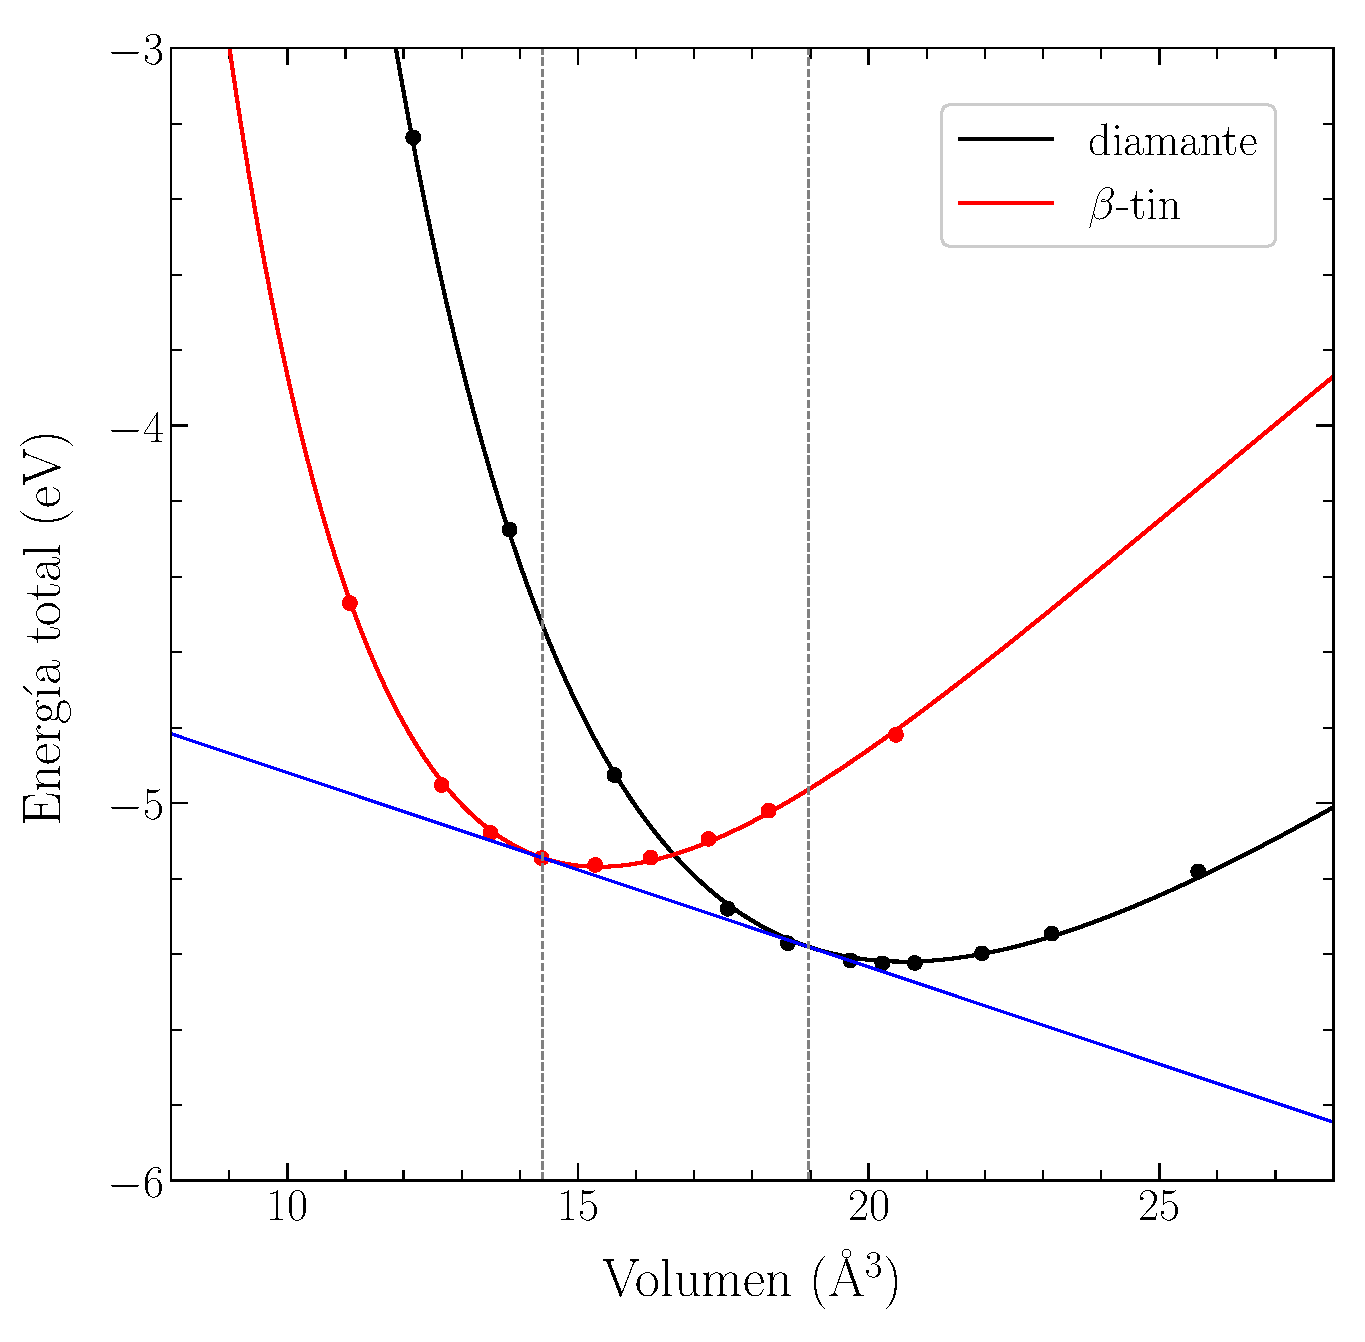
\includegraphics[width=0.4\textwidth]{Si/punto6.eps}
\end{figure}

\end{document}
